\documentclass[12pt]{article}
\usepackage{amsmath}
\usepackage{parskip}
\usepackage{graphicx}
\usepackage[letterpaper, margin=1in]{geometry}
\usepackage{fancyhdr}
\fancypagestyle{prelabheader} {
    \rhead{Raeed Hassan \\ hassam41}
    \lhead{\huge{ELECENG 2CI5 Lab 4 Prelab}}
}
\graphicspath{{./images/}}

\begin{document}
\newgeometry{margin=1in, includehead, head=47pt}
\thispagestyle{prelabheader}
i. \\
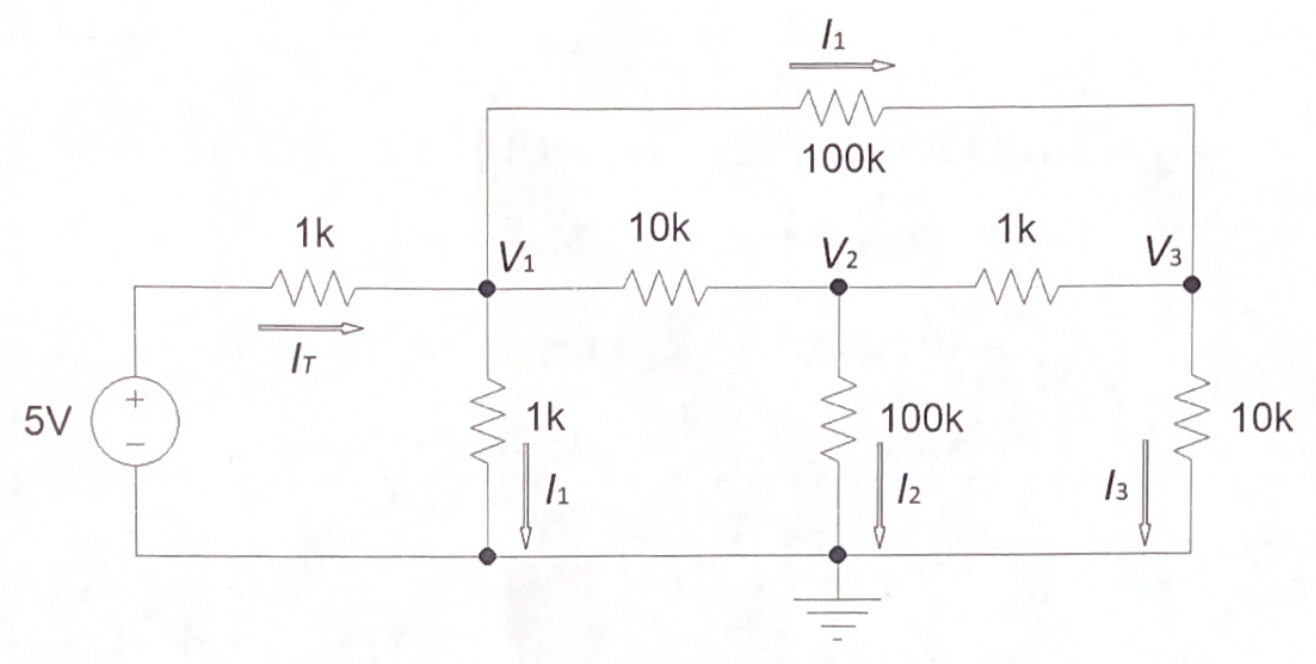
\includegraphics[width=\textwidth]{Circuit} \\

\underline{Node 1}
\begin{multline}
\frac{V_1}{1k} + \frac{V_1-V_2}{10k} + \frac{V_1-V_3}{100k} - \frac{V_1+5V}{1k} = 0 \\
100V_1 + 10V_1 + V_1 + 100V_1 - 10V_2 - V_3 - 500V = 0 \\
211V_1 - 10V_2 - V_3 = 500V
\end{multline}

\underline{Node 2}
\begin{multline}
\frac{V_2-V_1}{10k} + \frac{V_2-V_3}{1k} + \frac{V_2}{100k} = 0 \\
-10V_1 + 10V_2 + 100V_2 + V_2 - 100V_3 = 0 \\
-10V_1 + 111V_2 - 100V_3 = 0
\end{multline}

\underline{Node 3}
\begin{multline}
\frac{V_3}{10k} + \frac{V_3-V_2}{1k} + \frac{V_3-V_1}{100k} = 0\\
-V_1 - 100V_2 + 10V_3 + 100V_3 + V_3 = 0 \\
-V_1 - 100V_2 + 111V_3 = 0    
\end{multline}
\restoregeometry
\clearpage
\[
\begin{matrix}
    (1) \\
    (2) \\
    (3)    
\end{matrix}
\begin{bmatrix}
    211 & -10 & -1 \\
    -10 & 111 & -100 \\
    -1 & -100 & 111
\end{bmatrix}
\begin{bmatrix}
    V1 \\
    V2 \\
    V3
\end{bmatrix}
=
\begin{bmatrix}
    500 \\
    0 \\
    0
\end{bmatrix}
\]

\[
\begin{bmatrix}
    V1 \\
    V2 \\
    V3
\end{bmatrix}
=
\begin{bmatrix}
    2.4354 \\
    1.2696 \\
    1.1657
\end{bmatrix}
\]

\begin{gather*}
I_T = \frac{5V-V_1}{1k} = \frac{5-2.4354}{1k} = 0.002565A = 2.565mA \\
I_1 = \frac{V1}{1k} = \frac{2.4354}{1k} = 0.002435A = 2.435mA \\
I_2 = \frac{V2}{100k} = \frac{1.2696}{100k} = 0.01270mA \\
I_3 = \frac{V3}{10k} = \frac{1.1657}{10k} = 0.1166mA \\
I_4 = \frac{V_1-V_3}{100k} = \frac{2.4354-1.1657}{100k} = 0.01270mA 
\end{gather*}

ii. \\
$V_1$ = 2.554V \\
$V_2$ = 1.266V \\
$V_3$ = 1.160 V \\
$I_T$ = 2.558 mA \\
$I_1$ = 2.443 mA \\
$I_2$ = 0.01270 mA \\
$I_3$ = 0.1166 mA \\
$I_4$ = 0.01262 mA \\

iii. The ratio of the input voltage to $V_1$ is $\frac{5V}{2.554V} = 1.958V$, the ratio of the input voltage to $V_2$ is $\frac{5V}{1.266V} = 3.949V$, and the ratio of the input voltage to $V_3$ is $\frac{5V}{1.160V} = 4.310$. \\

\newpage

iv. \\
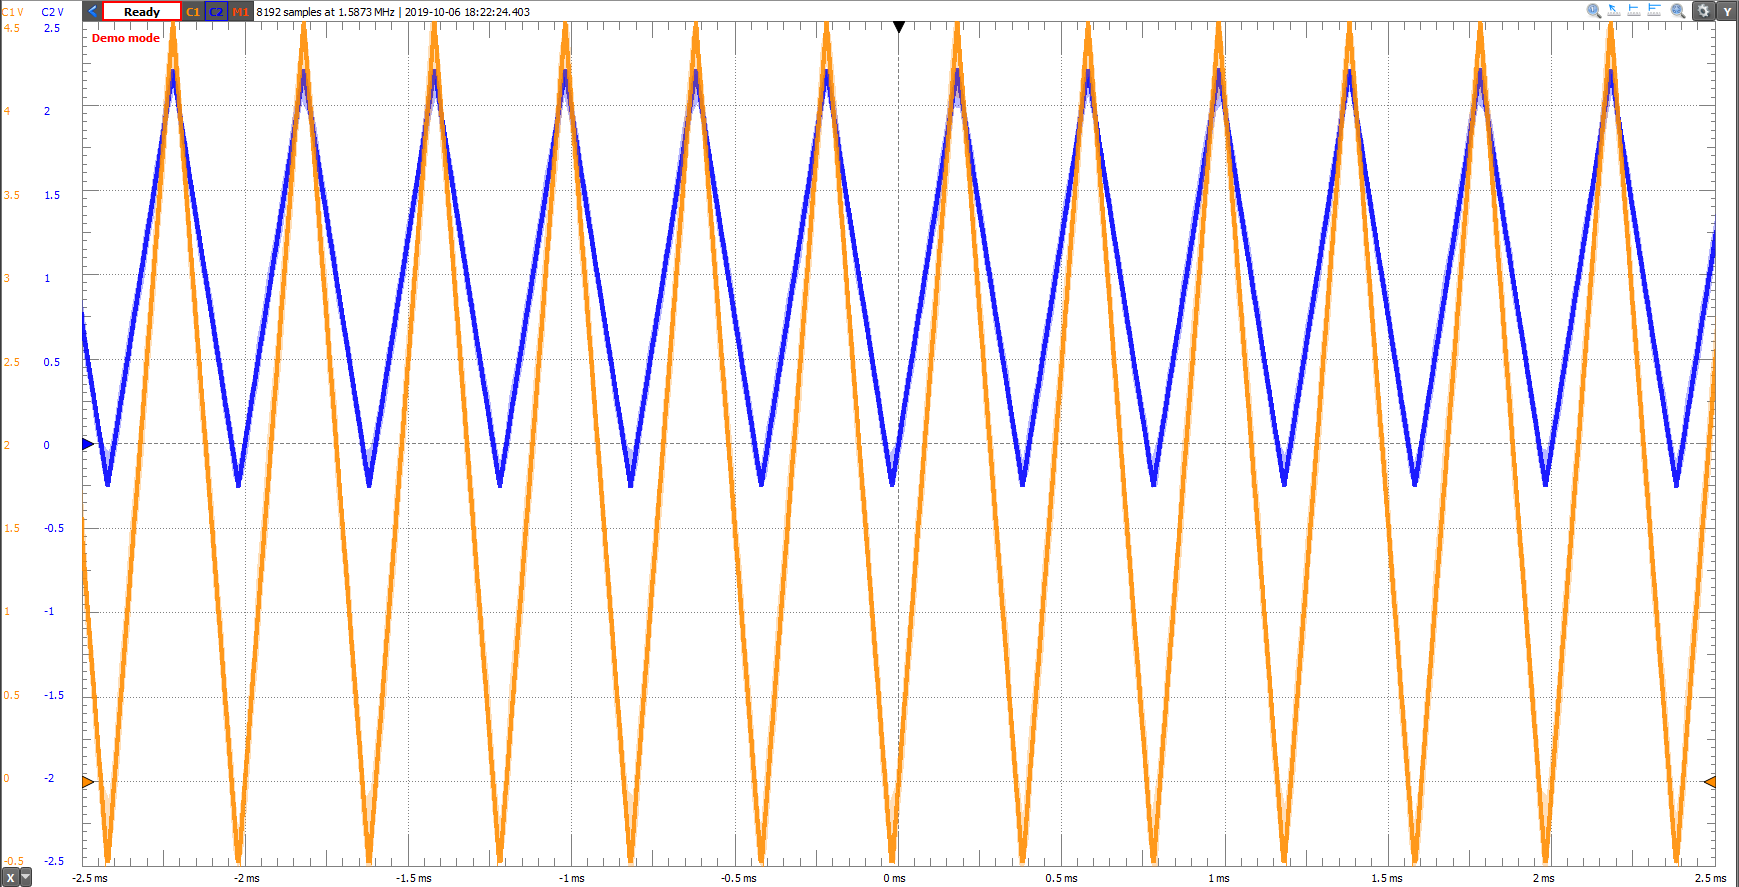
\includegraphics[width=\textwidth]{Q4.png} \\

v. \\
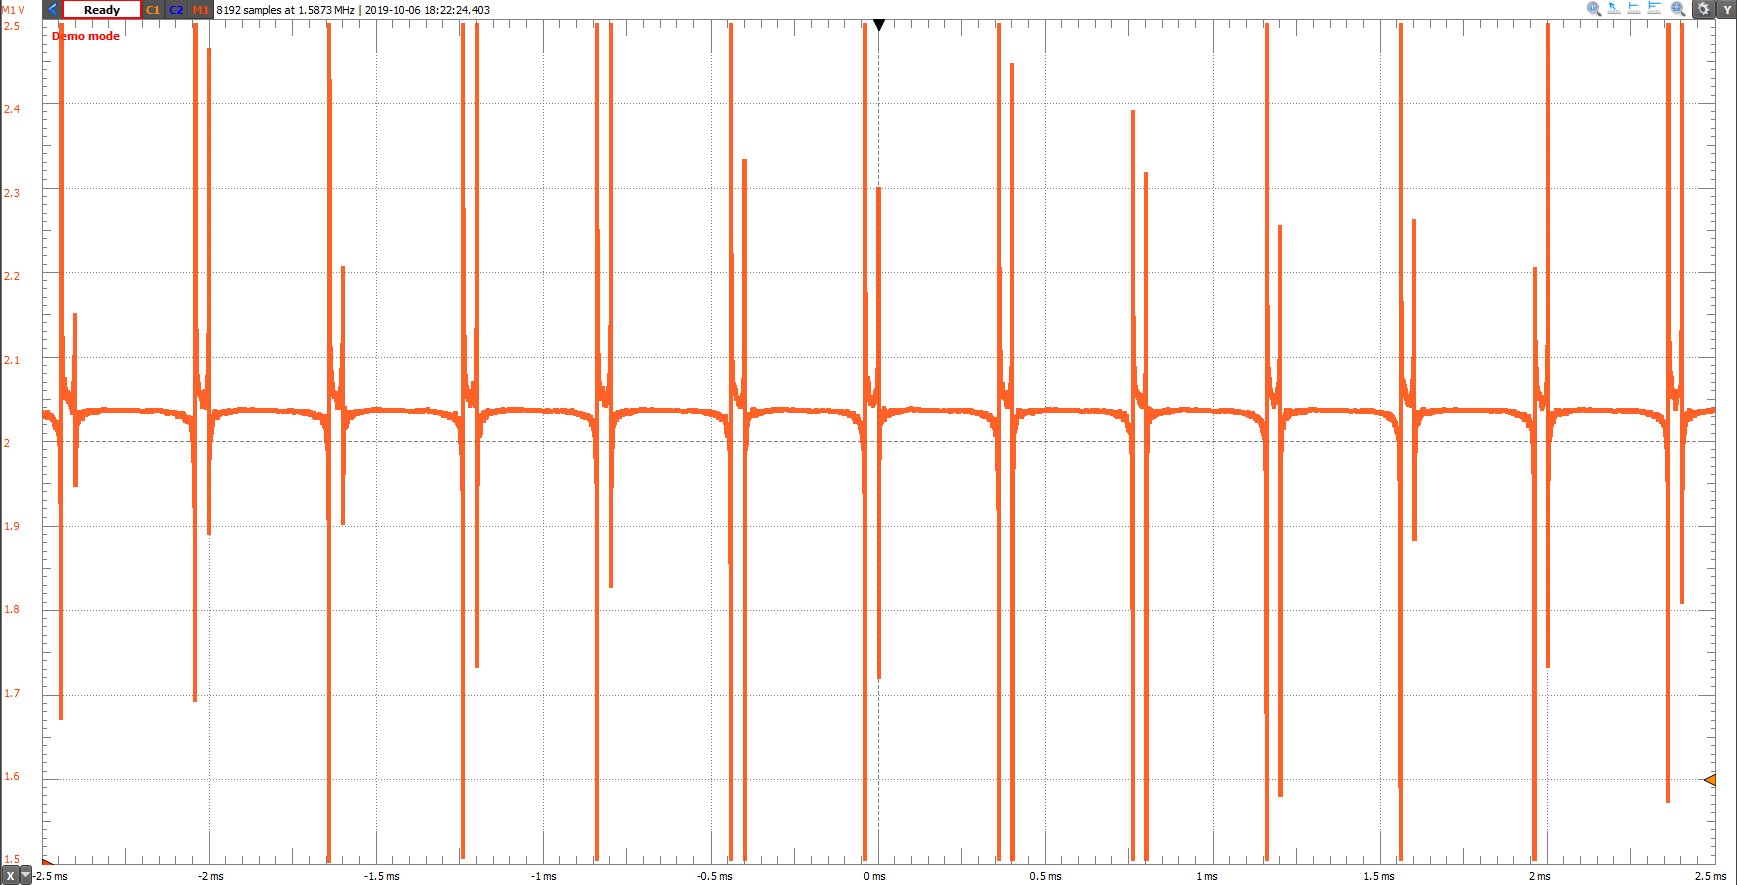
\includegraphics[width=\textwidth]{Q5.png} \\
The ratio displayed on the oscillioscope (approximately 2.05) is relatively close to the ratio calculated in part iii (approximately 1.96).

\end{document}